\documentclass[autodetect-engine,dvipdfmx-if-dvi,ja=standard,a4j,jbase=11pt,magstyle=nomag*]{bxjsreport}
% \documentclass[uplatex, dvipdfmx, a4paper, 11ptj, report]{jsbook}
% small japanese font size:     9pt, 10pt, 11pt, 12pt, 14pt, ... (please refer the document of jsclasses)
% word-like japanese font size: 10ptj 10.5ptj, 11ptj, 12ptj (or jbase=xxpt (without 'j') if error is occured)
    
\usepackage{ifptex,ifxetex,ifluatex}
\ifluatex
    \usepackage{bxcalcux}
    \ltjsetparameter{jacharrange={-2,-3}}
    \usepackage{luatexja-otf}
    \usepackage{bxbase}
\else\ifxetex
    % \usepackage{zxjatype}
    % \usepackage[macros]{zxotf}
    \XeTeXgenerateactualtext=1
    \usepackage{xltxtra}
    \usepackage{bxbase}
\else\ifuptex
    \usepackage{otf}
    \usepackage[prefernoncjk]{pxcjkcat}
    \cjkcategory{sym11,sym18,sym19}{cjk}
    \usepackage[utf8]{inputenc}
    \usepackage{pxbase}
\else\ifstrictptex
    \usepackage{otf}
    \usepackage[utf8]{inputenc}
    \usepackage{pxbase}
\fi\fi\fi\fi

\usepackage[LGR,T2A,T1]{fontenc}

\usepackage{graphicx}
% \usepackage[dvipdfmx]{graphicx}
\usepackage{grffile}

% paper layout setting
\setpagelayout{noheadfoot, left=18.0truemm, right=18.0truemm, top=29.0truemm, bottom=26.0truemm, columnsep=6.5truemm}
% \setpagelayout{noheadfoot, left=15.0truemm, right=5.0truemm, top=12.5truemm, bottom=12.5truemm, columnsep=5.0truemm}

% font setting
\usepackage{amsmath}
\usepackage{amssymb}
\usepackage{mathtools}
\usepackage{bm}
\usepackage{fix-cm}
\usepackage{newtxtext}
\usepackage[slantedGreek]{newtxmath}

% caption setting
\usepackage[font=bf,labelfont=bf,labelsep=quad]{caption}

% to balance the last page of the two-column article
% \usepackage[nospread, keeplastbox, nodebug]{flushend}

% title font style
\renewcommand{\headfont}{\bfseries}

% section setting (using titlesec, uelm package)
\renewcommand{\thesection}{\arabic{section}}
\renewcommand{\thesubsection}{\arabic{section}.\arabic{subsection}}

\usepackage[explicit]{titlesec}
\usepackage[normalem]{ulem}
\titleformat{name=\section}{\normalfont\headfont\normalsize\raggedright}{}{0pt}{\uline{\thesection.\quad#1}}
\titleformat{name=\section,numberless}{\normalfont\headfont\normalsize\raggedright}{}{0pt}{\uline{#1}}
% \titleformat{name=\section}{\normalfont\headfont\normalsize\raggedright}{}{0pt}{\thesection.\quad#1}
\titlespacing{name=\section}{0pt}{.5\Cvs plus .0\Cvs minus .3\Cvs}{.1\Cvs plus .0\Cvs minus .1\Cvs}
\titleformat{name=\subsection}{\normalfont\headfont\normalsize\raggedright}{}{0pt}{\thesubsection.\quad#1}
\titleformat{name=\subsection,numberless}{\normalfont\headfont\normalsize\raggedright}{}{0pt}{#1}
\titlespacing{name=\subsection}{0pt}{.3\Cvs plus .0\Cvs minus .2\Cvs}{.0\Cvs plus .0\Cvs minus .0\Cvs}

% \makeatletter
% \renewcommand{\section}{\@startsection{section}{1}{\z@}{.5\baselineskip}{.1\baselineskip}{\normalfont\normalsize\headfont\raggedright}}
% \renewcommand{\subsection}{\@startsection{subsection}{2}{\z@}{.3\baselineskip}{\z@}{\normalfont\normalsize\headfont\raggedright}}
% \makeatother

\usepackage{secdot}
\sectiondot{section}
\sectiondot{subsection}

% list (itemize, enumerate, description, ...)
\usepackage{enumitem}
\setlist[1]{parsep=.0\baselineskip,topsep=.2\baselineskip,itemsep=.1\baselineskip}
% \makeatletter
% \def\@listi{\leftmargin\leftmargini
%     \parsep \z@
%     \topsep .2\baselineskip
%     \itemsep .1\baselineskip \relax}
% \let\@listI\@listi
% \makeatother

% no page number
\pagestyle{empty}

% footnote
\usepackage[bottom,hang,stable]{footmisc}
\setlength{\footnotemargin}{0pt}

% float setting (figure, table)
\setlength\floatsep{2.0truemm}
\setlength\textfloatsep{2.0truemm}
\setlength\intextsep{1.0truemm}
\setlength\dblfloatsep{2.0truemm}
\setlength\dbltextfloatsep{2.0truemm}
\setlength\abovecaptionskip{0.5truemm}
\setlength\belowcaptionskip{0.5truemm}

% lineskip setting (body text, display-style equation)
\AtBeginDocument{%
    \narrowbaselines    % basic english lineskip (for article)
    % \widebaselines      % basic japanese lineskip
    %
    \setlength\abovedisplayskip{1.5truemm}    % equation setting
    \setlength\belowdisplayskip{1.5truemm}    % equation setting
}

% to suit ms-word template
\renewcommand{\baselinestretch}{0.9}


\makeatletter
%
% maketitle
% additional elements
\newcommand*{\etitle}[1]{\gdef\@etitle{#1}}
\newcommand*{\studentid}[1]{\gdef\@studentid{#1}}
\newcommand*{\laboarea}[1]{\gdef\@laboarea{#1}}
\newcommand*{\laboname}[1]{\gdef\@laboname{#1}}
%
% style definition
\def\@maketitle{%
\newpage%
\centering%
\let\footnote\thanks%
%
% title
{\fontsize{16.00truept}{16.00truept}\selectfont\headfont\@title\par}%
%
% english title
\ifx\@etitle\@undefined\else{\vspace{1truemm}{\fontsize{12truept}{12truept}\selectfont\headfont\@etitle\par}}\fi%
%
% name (option: student id)
\vspace{1truemm}%
\ifx\@studentid\@undefined\else{\fontsize{12truept}{12truept}\selectfont\headfont\@studentid\hspace{\Cwd}}\fi%
{\fontsize{12truept}{12truept}\selectfont\headfont\@author\par}%
%
% research area (\laboarea) and laboratory name (\laboname)
\ifx\@laboarea\@undefined%
    \ifx\@laboname\@undefined%
    \else\vspace{1truemm}{\fontsize{12truept}{12truept}\selectfont\headfont\@laboname\par}%
    \fi%
\else%
    \ifx\@laboname\@undefined\vspace{1truemm}{\fontsize{12truept}{12truept}\selectfont\headfont\@laboarea\par}%
    \else\vspace{1truemm}{\fontsize{12truept}{12truept}\selectfont\headfont\@laboarea\hspace{\Cwd}\@laboname\par}%
    \fi%
\fi%
%
%% old version (2 line) of research area (\laboarea) and laboratory name (\laboname)
%\ifx\@laboarea\@undefined\else{\vspace{1truemm}{\fontsize{10truept}{10truept}\selectfont\@laboarea\par}}\fi%
%\ifx\@laboname\@undefined\else{\vspace{1truemm}{\fontsize{10truept}{10truept}\selectfont\@laboname\par}}\fi%
%
%% date (error)
% \ifvoid\@date\else{\vspace{2truemm}{\fontsize{12truept}{12truept}\selectfont\@date\par}}\fi%
%
% abstract (no check)
\ifvoid\@abstractbox\else{\vspace{2truemm}{\centering{\fontsize{10truept}{10truept}\selectfont\box\@abstractbox\par}}}\fi%
\vspace{2truemm}%
}
%
%
% bibliography
\newcommand{\@bibsection}{\@startsection{section}{1}{\z@}{.5\baselineskip}{0.2\baselineskip}{\normalfont\fontsize{9truept}{11truept}\selectfont\headfont\raggedright}}
\setlength\bibindent{\Cwd}
\renewenvironment{thebibliography}[1]{%
    \global\let\presectionname\relax
    \global\let\postsectionname\relax
    \@bibsection*{\refname}\@mkboth{\refname}{\refname}%
    \list{\@biblabel{\@arabic\c@enumiv}}{%
        \settowidth\labelwidth{\@biblabel{#1}}%
        \leftmargin\labelwidth
        \advance\leftmargin\labelsep
        \setlength\itemsep{0.5truept plus 1.0truept minus 0.5truept}
        \@openbib@code
        \usecounter{enumiv}%
        \let\p@enumiv\@empty
        \renewcommand\theenumiv{\@arabic\c@enumiv}}%
    \fontsize{8truept}{9.5truept}\selectfont
    \sloppy
    \clubpenalty4000
    \@clubpenalty\clubpenalty
    \widowpenalty4000%
    \sfcode`\.\@m}
{\def\@noitemerr{\@latex@warning{Empty `thebibliography' environment}}\endlist}
%
\makeatother


\mainmatter
\setchapterxr[thesis][bibliography]{2}


\begin{document}


\chapter[地上固定LiDARと複数UAVを用いた撮影計画の概要]{地上固定LiDARと複数UAV\\を用いた撮影計画の概要}

\section{はじめに}
本章では,昨年度まで佐々木らが行っていた地上固定LiDARと複数UAVを用いた撮影計画の概要に
ついて述べる.\cite{sasaki_2019}
またその研究における問題点,課題点などについて述べる.

\section{撮影ベクトルと移動カメラの撮影領域}
\subsection{撮影ベクトル}
カメラで撮影対象を撮影するとき,撮影対象の表面に対して垂直な方向から撮影することが望ましい.
撮影対象の表面に垂直な方向を撮影ベクトルと定義する.
また定義した撮影ベクトルに対して,一定の解像度以上で撮影できる領域を撮影領域と定義する.
要求解像度とUAVに搭載されている移動カメラの性能から撮影領域は計算できる.

撮影領域の導出において,三次元空間および二次元空間はグリッドによって分割され,
それぞれボクセル,セルとして管理される.\cref{fig:voxel}は撮影対象人物とその人物に対するボクセルと撮影ベクトルである.
この研究では\cref{fig:voxel}で中心のセルから撮影ベクトルが表されているように,
簡単のため,対象人物をは1つのボクセル内で存在するものとし,
その1つのボクセルから垂直な方向に撮影ベクトルを定義する.

\begin{figure}[t]
    \centering
    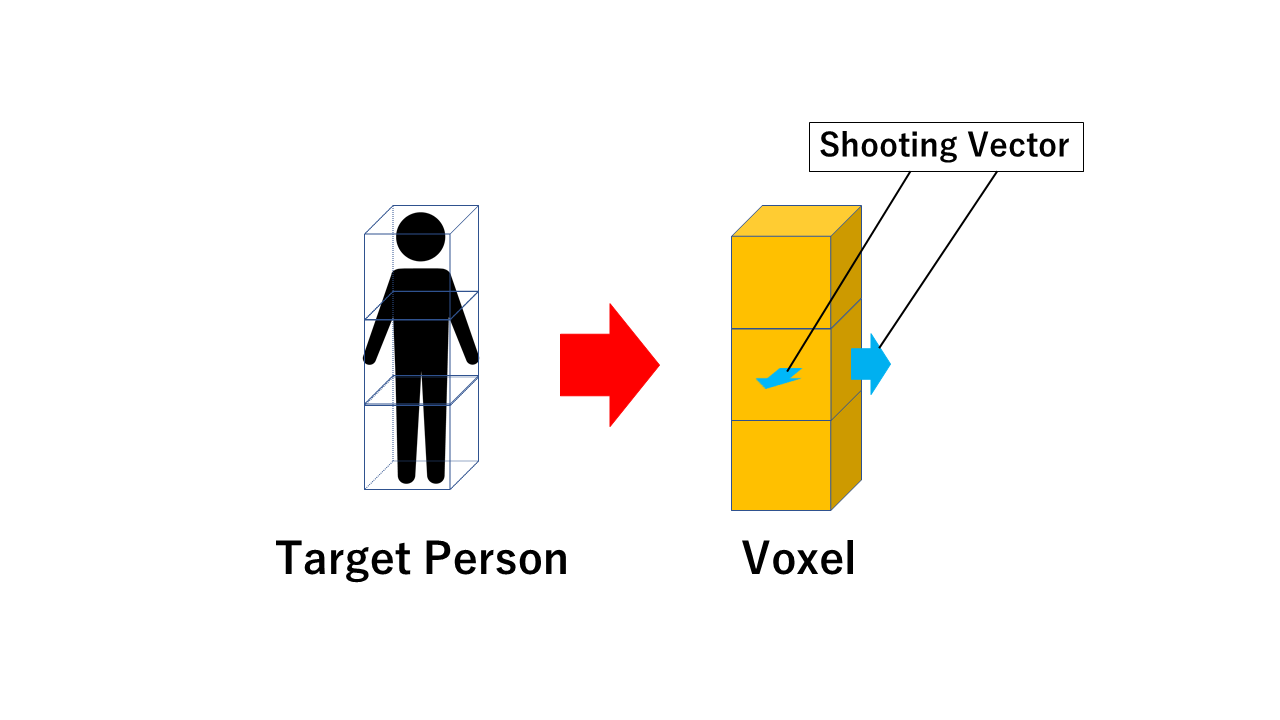
\includegraphics[width=\linewidth, clip]{./figure/chapter2/voxel.png}
    \caption{Model of Shooting Vector}
    \label{fig:voxel}
\end{figure}

\subsection{要求解像度}
この研究では,1[mm]を表すために必要な画素数[pixel/mm]で解像度を表現する.
あるカメラが撮影対象を撮影しているとき,カメラの水平(垂直)解像度を$R_{camera}$,
カメラの水平(垂直)画角を$\alpha$[rad],撮影対象を写している水平(垂直)画角を$\beta$とし,
セルの1辺の長さが$S$[mm]であるときの,撮影対象の解像度$R$[pixel/mm]は\cref{eq:pixel_mm}
で求められる.

\begin{equation}
    \label{eq:pixel_mm}
    \begin{aligned}
        \frac{\beta R_{camera}}{\alpha S}\mathrm{[pixel/mm]}
    \end{aligned}
\end{equation}

任意の要求解像度$n$[pixel/mm]が与えられたとき,要求解像度の満たすための条件は
\cref{eq:pixel_mm}より$n \le R$で表される.
この式より,要求解像度を満たすためには画角$\beta$に対して\cref{eq:angle_rule}を満足する必要がある.

\begin{equation}
\beta \le \frac{\alpha n S}{R_{camera}}\mathrm{[rad]}
\label{eq:angle_rule}
\end{equation}

以上より,ある撮影ベクトルについて要求解像度を満たす撮影領域は,
条件\cref{eq:angle_rule}を満たす水平画角$\beta_h$,垂直画角$\beta_v$の点の軌跡である.

\subsection{撮影領域の導出}
撮影領域の導出を平面について順番に導出していく.まず始めにx,y平面について考える.
撮影ベクトルが設定されたセルの中心を原点とするx,y座標系を考える.カメラの座標を($x$,$y$)[mm],撮影ベクトルとx軸のなす角を$\gamma$,セルの1辺の長さを2$\lambda$[mm]とすると水平画角$\beta_h$はのようになる.

\begin{equation}
\beta_{h}=\left|\arctan \left(\frac{y+\lambda \cos \gamma}{x-\lambda \sin \gamma}\right)-
               \arctan \left(\frac{y-\lambda \cos \gamma}{x+\lambda \sin \gamma}\right)\right|
\label{eq:beta_h_1}
\end{equation}

簡単のために$\gamma=0$のときを考えると,xy平面における水平画角$\beta_h$で捉えることのできる点の軌跡は
\cref{eq:beta_h_2}のようになる.

\begin{equation}
    \begin{aligned}
    \left(  x - \frac{\lambda}{\tan \beta_{h}}  \right) ^2 + y^2 & = \left( \frac{\lambda}{\tan \beta_{h}} \right) ^2 + \lambda^2
    \end{aligned}
\label{eq:beta_h_2}
\end{equation}

この式を極座標形式に変換すると\cref{eq:beta_3}になる.

\begin{equation}
r(\phi)=\frac{\cos \phi+\sqrt{\cos^{2}\phi+\tan^{2}\beta_{h}}}{\tan \beta_{h}}\, \lambda
\label{eq:beta_h_3}
\end{equation}

zr平面について考える.xy平面の時と同様に,セルの中心を原点とする座標系を考える.
カメラの位置を$z$,$r(\phi)$[mm],撮影ベクトルとr軸のなす角を$\psi$[rad],
セルの$1$辺の半分を$\lambda$[mm]とする.
撮影対象を捉えている垂直画角$\beta_{v}$は,\cref{eq:beta_v_1}のようになる.

\begin{equation}
\beta_{v}=\left|\arctan \left(\frac{z+\lambda \cos \psi}{r(\phi)-\lambda \sin \psi}\right)-
               \arctan \left(\frac{z-\lambda \cos \psi}{r(\phi)+\lambda \sin \psi}\right)\right|
\label{eq:beta_v_1}
\end{equation}

xy平面のとき同様に,$tan$に変形すると,\cref{eq:beta_v_2}のようになる.


\begin{equation}
\tan \beta_{v}=\frac{2r(\phi)\lambda \cos \psi + 2z\lambda \sin \psi}{z^2 + r(\phi)^2 - \lambda^2}
\label{eq:beta_v_2}
\end{equation}

簡単のために,$\psi = 0$の時を考えると,zr平面における撮影ベクトルを捉えるために必要な垂直画角$\beta_{v}$[rad]で捉えることのできる点の軌跡は,
\cref{eq:beta_v_3}のようになる.

\begin{equation}
    \begin{aligned}
    z^2 + r(\phi)^2 + \lambda^2 & = \frac{2r(\phi) \lambda}{\tan \beta_{v}} \\ 
    z^2 + \left(  r(\phi) - \frac{\lambda}{\tan \beta_{v}}  \right) ^2  & = \left( \frac{\lambda}{\tan \beta_{v}} \right) ^2 + \lambda^2
    \end{aligned}
\label{eq:beta_v_3}
\end{equation}

上式をz軸方向を$\theta$の正とした距離$r$,角度$\theta$による$3$次元極座標系の式に変形し,$r(\theta, \phi)$について解くと
\cref{eq:shooting_area}となる.
\begin{equation}
r \left (\theta, \phi \right ) \le \lambda^2 \left \{ \left (\frac{\sin\theta+\sqrt{\sin^2\theta + \tan^2\beta_v}}{\tan\beta_v \cos\theta} 
- \frac{\cos\phi}{\tan\beta_h} \right )^2 + \left (\frac{\sin\phi}{\tan\beta_v} \right )^2 \right \}
\label{eq:shooting_area}
\end{equation}

\cref{eq:shooting_area}と\cref{eq:angle_rule}を合わせた条件を満足する位置が撮影領域である.

\subsection{カメラの高さや向きを考慮した撮影領域の算出}
この研究ではUAVの高度を一定にして実験を行っている.そのときのUAVの高度を$h$[mm]とするとその時の\cref{eq:shooting_area}に課される拘束条件は
\cref{eq:shooting_area_2d}になる.
次にカメラのロール,ピッチ,ヨーの可動域を考える.ピッチを$\omega$[rad]で固定した場合,ヨー,ピッチを,$\mu$,$\omega$[rad]とし
,$\mu$,$\omega$,$\phi$,$\theta$およびカメラの水平画角$\alpha_h$と垂直画角$\alpha_v$に関して,\cref{eq:shooting_area_gimbal}の拘束条件が課される.

\begin{equation}
    \begin{aligned}
    \mathrm{subject~to} \,\, r(\theta, \phi) \cos \theta = h
    \end{aligned}
\label{eq:shooting_area_2d}
\end{equation}

\begin{equation}
    \begin{aligned}
    \mathrm{subject~to} \,\, |\phi| \le \mu +  \frac{\alpha_h}{2}, \,\, \omega - \frac{\alpha_v}{2} \le \theta \le \omega + \frac{\alpha_v}{2}
    \end{aligned}
\label{eq:shooting_area_gimbal}
\end{equation}

\subsection{1人の撮影人物に対して設定する撮影ベクトルの本数}
前節では撮影ベクトルの領域の導出をしたが,その領域は1つの撮影ベクトルの方向のみ補完している.
実際に人物認識を行うためには,対象人物の周囲の領域を全てフォローする必要がある.
その条件を満たすために1人の人物に複数本の撮影ベクトルを付与する.
1つのセルから出る撮影ベクトルの本数が4本であることを考慮すると,撮影ベクトルの本数は4の倍数であることが望ましい.

\section{UAVの目標位置の導出}
\subsection{グリッドマップと目標位置}
本研究では,人物移動領域とUAV移動可能領域をグリッドマップで管理する.
人物移動領域で認識された人物と前節までに導出した撮影ベクトルの領域からUAVの移動可能位置における目標位置の投票を行う.
撮影人物に付与された撮影ベクトルをグリッドマップに投影し,撮影ベクトルの領域に含まれるグリッドマップのセルがUAVの目標位置になる.
実際には撮影人物は複数人存在し1人に対して撮影ベクトルは複数本付与されているため,
UAVの目標位置は撮影ベクトルがある領域のうち,撮影ベクトルがより多く重なっているセルである.
移動カメラが現在いる位置から次の目標位置を受け取るまでに動くことができる距離には制限がある.
移動カメラの最大並進速度を$v_{max}$[m/s],撮影計画の実行周期を$f_{plan}$[Hz]とすると,
1周期内で移動カメラが移動できる最大並進距離$d_{max}$[m]は,\cref{eq:camera_max_distance}のようになる.

\begin{equation}
d_{max} = \frac{v_{max}}{f_{plan}}
\label{eq:camera_max_distance}
\end{equation}

移動カメラの現在位置を中心とし$d_{max}$を半径とする円が,実行周期内にUAVの移動できる領域になる.
この円の中にあり撮影ベクトルが一番多く重なっているグリッドマップのセルがUAVの目標位置である.

\section{先行研究の課題点と本章のまとめ}
前節までに導出した撮影ベクトルの設定やUAVの目標位置決定の導出の手法を使ってUAV撮影計画を行っていたが,実機実験では様々な問題点が発生していた.

UAVのGPSセンサの精度が低く,目標位置に移動する際に実際の目標位置とUAVが到達した目標位置にずれが生じる.
またLiDARの位置情報をUAVに搭載されているGPSセンサと同じものを用いて取得しているため,LiDARが認識している人物の位置の精度が低い.
LiDARに対して撮影対象が複数人いる場合に遮蔽(オクルージョン)が発生する.オクルージョンが発生した場合,
位置情報が取得できない人物が存在するため撮影ベクトルの本数が減少し,UAVの目標位置が人物を捉えきれない位置に設定されることがある.

次章ではLiDARの精度の高い位置の決定方法とオクルージョンが発生した場合のUAVの目標位置の補完方法について述べる.

\section{制約条件}


\subsection{地形との接触制約}




\subsection{遊脚の配置制約}


\subsection{脚先の干渉防止制約}


\subsection{二次計画問題への適用}


\section{本章のまとめ}
本章では,三次元適応のための歩行モデルの拡張および追加の制約条件について説明した.
従来の水平方向の脚配置計画のためのモデルに,独立した垂直方向の動作を追加し,
脚配置遷移モデルの状態および入力についての次元の拡張を行うことなく,
事前に与えられた地形情報に基いて垂直方向の移動量を制限する制約を定式化し追加することで,
計算コスト増加を抑えつつ三次元地形への適応を可能にした.
次章では,本章で定義した計画問題の解法について,
全体のアルゴリズムおよび求解性能の安定化のためのいくつかの手法について述べる.


\end{document}
